\documentclass[11pt,a4paper]{article}

\usepackage[margin=2.3cm]{geometry}
\usepackage{amsmath,amssymb}
\usepackage{graphicx}
\usepackage{booktabs}
\usepackage{xcolor}
\usepackage{enumitem}
\usepackage[hidelinks]{hyperref}
\usepackage{caption}

\emergencystretch=1.5em
\captionsetup{font=small,labelfont=bf,width=.92\textwidth}
\setlength{\parskip}{4pt plus 1pt}
\setlength{\parindent}{0pt}

\newcommand{\code}[1]{\texttt{#1}}
\newcommand{\bst}[1]{\textbf{#1}}
\newcommand{\Kp}{K'}

\title{The soft-forward bottleneck\\[2pt]
\large Research note: \code{rblapsum\_sf} against its hard-forward twin and the
hard Top-$\Kp$ ladder}
\author{}
\date{2026-09-27.}

\begin{document}
\maketitle
\vspace{-2em}

% ============================================================
\section{Purpose and summary of conclusions}
% ============================================================

\code{rblapsum\_sf} keeps RBLapSum's Top-$(K{+}J)$ candidate pool, rank
boundary $b = \max(b_0, s_{(K+1)})$ and exponential kernel, but places the
probabilities in the forward pass: every pool member outputs
$z_i\,p_i$ with $p_i = F\!\big((s_i - b)/T\big)$ (the Laplace CDF), features
outside the pool output exactly zero, and the backward pass is the gradient of
this forward -- there is no train-time discrepancy between the function
trained and the function differentiated. The boundary's own derivative is
routed by the same switch as in the hard-forward mode and is
$\kappa$-weighted (\code{through\_rank\_kappa}) throughout this note.

Because the trained forward is soft, two validation metrics exist and they
disagree strongly. \code{val/ce} evaluates the model under the hard Top-$K$
forward that every other regime uses at inference (only the $K$ selected
activations participate), and is directly comparable across regimes.
\code{val\_soft/ce} evaluates the soft forward actually trained. This note
reports both, against two references: the hard-forward
\code{through\_rank\_kappa} twin of every cell, and the hard Top-$\Kp$
post-norm baselines at the matching pool $\Kp = K+J$.

Conclusions:

\begin{itemize}[leftmargin=1.4em]
\item \textbf{Under its own forward, the soft model beats the hard Top-$\Kp$
baseline with the same pool in every cell}, by $0.055$ to $0.114$ nats. The
best values are the best in the project so far: $1.3430$ at $(K,J)=(64,448)$
and $1.3498$ at $(32,480)$, both at $T=2$, against $1.4232$ for hard Top-512
and $1.4146$ for the best hard-forward surrogate cell.

\item \textbf{Under the hard Top-$K$ forward, the soft model loses to its
hard-forward twin in every cell}, by $0.086$ to $1.14$ nats, and widening $J$
makes it monotonically worse -- the opposite of the hard-forward family, where
widening $J$ helps. The damage tracks the probability mass the trained
forward carries outside the top $K$ (measured below).

\item \textbf{The two metrics invert every ordering the earlier campaigns
established.} Under soft evaluation: widening $J$ helps monotonically with no
reversal at $(32,480)$; $T=2$ is better than the post-norm in eight of nine
comparable cells (they are equal within $0.001$ at $(128,384)$); and at a
fixed pool the active count $K$ barely matters -- the spread across $K$ is
$0.006$--$0.020$ nats, an order of magnitude smaller than the pool effect.

\item \textbf{Stability is not improved.} One cell diverged: $(128,128)$ at
$T=2$, stopped by the guard at step 3480, a cell whose hard-forward twin
survives. $(128,384)$ at $T=2$ had a large recovered excursion near step
7000. The post-norm arm survived everywhere.

\item \textbf{As a route to a hard Top-$K$ model, the soft forward currently
pays for itself}: the smallest hard-eval penalty in the grid is $+0.086$
nats at $(256,256)$ post-norm. As a model evaluated the way it is trained --
a weighted pool of $K{+}J$ features -- it is the strongest configuration
tested in this project at every pool size.
\end{itemize}

% ============================================================
\section{Setup}
% ============================================================

Twenty runs: the ten $(K,J)$ cells of the Top-$(K{+}J)$-versus-hard note
($K, K{+}J \in \{32,64,128,256,512\}$, $J = \Kp - K > 0$), each under the two
variants of that note -- $T=2$ with no output norm, and $T=1$ with an RMSNorm
on each bottleneck's output (``post-norm''). Every run inherits the dumped
\code{config.json} of its hard-forward \code{through\_rank\_kappa} twin (the
stabilization campaign for the six cells trained there, the Top-$(K{+}J)$
campaign for the rest), with only the surrogate mode overridden: architecture,
data, optimizer, schedules, seed, $b_0 = 0$ and the support scale $1.0$ are
identical by construction. Divergence guard as in the earlier campaigns.

The two references. The hard-forward twins' curves are the original runs of
their campaigns. The hard Top-$\Kp$ post-norm baselines are the same five runs
used in the Top-$(K{+}J)$ note. Both were recovered from the Drive backups of
the retired machine; the new runs trained on the successor box from the same
repo state.

Evaluation. \code{val/ce} is computed with \code{hard\_inference}: the
forward keeps the top $K$ activations and drops the rest, exactly the
inference forward of every other regime, so the number is comparable on the
same TensorBoard plot. \code{val\_soft/ce} is a second evaluation pass with
the trained soft forward, $z_i p_i$ over the pool. The training-side
\code{active\_count} (L0) remains the hard support size $K$; the pool's
probability mass $\sum_i p_i$ is logged as \code{rb\_soft\_mass}.

% ============================================================
\section{Results}
% ============================================================

\subsection*{Hard evaluation: the comparable metric}

Final \code{val/ce} after 20k steps, soft-forward (sf) against its
hard-forward twin (kappa):

\begin{center}\small
\begin{tabular}{lcccccc}
\toprule
& \multicolumn{3}{c}{$T=2$} & \multicolumn{3}{c}{post-norm} \\
\cmidrule(lr){2-4}\cmidrule(lr){5-7}
$(K,J)$ & kappa & sf & gap & kappa & sf & gap \\
\midrule
$(32,32)$   & 1.5492 & 1.6815 & $+0.132$ & 1.5310 & 1.6574 & $+0.126$ \\
$(32,96)$   & 1.5146 & 1.9369 & $+0.422$ & 1.5115 & 1.8368 & $+0.325$ \\
$(32,224)$  & 1.4842 & 2.2553 & $+0.771$ & 1.4949 & 2.0165 & $+0.522$ \\
$(32,480)$  & 1.4943 & 2.6381 & $+1.144$ & 1.5370 & 2.1118 & $+0.575$ \\
$(64,64)$   & 1.5142 & 1.6450 & $+0.131$ & 1.4834 & 1.6005 & $+0.117$ \\
$(64,192)$  & 1.4922 & 1.8927 & $+0.401$ & 1.4602 & 1.7563 & $+0.296$ \\
$(64,448)$  & 1.4727 & 2.1958 & $+0.723$ & 1.4538 & 1.9166 & $+0.463$ \\
$(128,128)$ & 1.4802 & \multicolumn{2}{c}{diverged (3480)} & 1.4423 & 1.5441 & $+0.102$ \\
$(128,384)$ & 1.4598 & 1.8537 & $+0.394$ & 1.4294 & 1.6954 & $+0.266$ \\
$(256,256)$ & 1.4425 & 1.8550 & $+0.413$ & 1.4146 & 1.5008 & $+0.086$ \\
\bottomrule
\end{tabular}
\end{center}

The soft model loses everywhere under this metric, the loss grows with $J$ at
every $K$, and it shrinks with $K$ at fixed $J/K$. The post-norm variant is
uniformly less damaged than $T=2$.

\subsection*{Soft evaluation: the trained function}

Final \code{val\_soft/ce}, grouped by pool, against hard Top-$\Kp$ with the
same pool (post-norm, hard evaluation -- its trained forward):

\begin{center}\small
\begin{tabular}{llcccc}
\toprule
pool $\Kp$ & $(K,J)$ & sf $T{=}2$ & sf post-norm & hard Top-$\Kp$ & best margin \\
\midrule
$64$  & $(32,32)$   & \bst{1.4269} & 1.4511 & 1.5408 & $-0.114$ \\
\midrule
$128$ & $(32,96)$   & \bst{1.3852} & 1.4054 & 1.4938 & $-0.109$ \\
      & $(64,64)$   & 1.3913 & 1.4039 & & $-0.103$ \\
\midrule
$256$ & $(32,224)$  & \bst{1.3645} & 1.3931 & 1.4560 & $-0.092$ \\
      & $(64,192)$  & 1.3667 & 1.3736 & & $-0.089$ \\
      & $(128,128)$ & --- & 1.3762 & & $-0.080$ \\
\midrule
$512$ & $(32,480)$  & 1.3498 & 1.3846 & 1.4232 & $-0.073$ \\
      & $(64,448)$  & \bst{1.3430} & 1.3633 & & $-0.080$ \\
      & $(128,384)$ & 1.3630 & 1.3624 & & $-0.060$ \\
      & $(256,256)$ & 1.3571 & 1.3653 & & $-0.066$ \\
\bottomrule
\end{tabular}
\end{center}

Every cell beats the pool-matched hard baseline. Within a pool the spread
across $K$ is small ($0.006$ at pool 128, $0.012$ at 256, $0.020$ at 512),
and the smallest $K$ is never the worst; the pool size dominates. $T=2$ is
ahead of the post-norm in every comparable cell except $(128,384)$, where the
two agree within $0.001$.

\subsection*{Where the hard-eval damage comes from}

\code{rb\_soft\_mass} $= \sum_i p_i$ over the pool at the end of training,
minus $K$, is the probability mass the trained forward carries outside the
kept set -- the part the hard evaluation deletes. Post-norm variant:

\begin{center}\small
\begin{tabular}{lccc}
\toprule
$(K,J)$ & mass $-\,K$ & hard-eval gap to kappa & gap per unit mass \\
\midrule
$(32,32)$   & 2.9  & $+0.126$ & 0.043 \\
$(32,96)$   & 9.3  & $+0.325$ & 0.035 \\
$(32,224)$  & 18.2 & $+0.522$ & 0.029 \\
$(32,480)$  & 30.9 & $+0.575$ & 0.019 \\
$(64,64)$   & 5.0  & $+0.117$ & 0.023 \\
$(64,192)$  & 18.5 & $+0.296$ & 0.016 \\
$(64,448)$  & 36.9 & $+0.463$ & 0.013 \\
$(128,128)$ & 9.6  & $+0.102$ & 0.011 \\
$(128,384)$ & 33.6 & $+0.266$ & 0.008 \\
$(256,256)$ & 17.3 & $+0.086$ & 0.005 \\
\bottomrule
\end{tabular}
\end{center}

Within each $K$ the gap grows monotonically with the tail mass; across $K$
the damage per unit of tail mass falls roughly as $1/K$, consistent with each
deleted feature mattering less when more are kept. The $T=2$ variant carries
$1.0$--$2.0\times$ more tail mass than the post-norm in every cell (e.g.\
$92.8$ vs $30.9$ at $(32,480)$), matching both its better soft and worse hard
evaluation.

\subsection*{Stability}

$(128,128)$ at $T=2$ diverged: best CE $1.74$ at step $\sim$3100, then a
gradient-norm blowup to $\sim 10^{11}$, stopped by the guard at 3480 after
300 steps above CE 7. Its hard-forward twin survives the same cell (final
$1.4802$), so the soft forward is not a stabilization. $(128,384)$ at $T=2$
burst near step 6500--7500 and recovered (visible in the pool-512 figure).
All ten post-norm cells and the remaining $T=2$ cells reached 20k steps.

\subsection*{Figures}

Each pool figure: left $T=2$, right post-norm; the hard-forward family in
blues, the soft-forward family in oranges, both light to dark with increasing
$K$; hard Top-$\Kp$ dashed black. The vertical axis is the hard-eval
\code{val/ce}, so these figures show the comparable metric; the soft-eval
figure that follows them shows \code{val\_soft/ce} for the soft family
against the same hard ladder.

\begin{figure}[htb]\centering
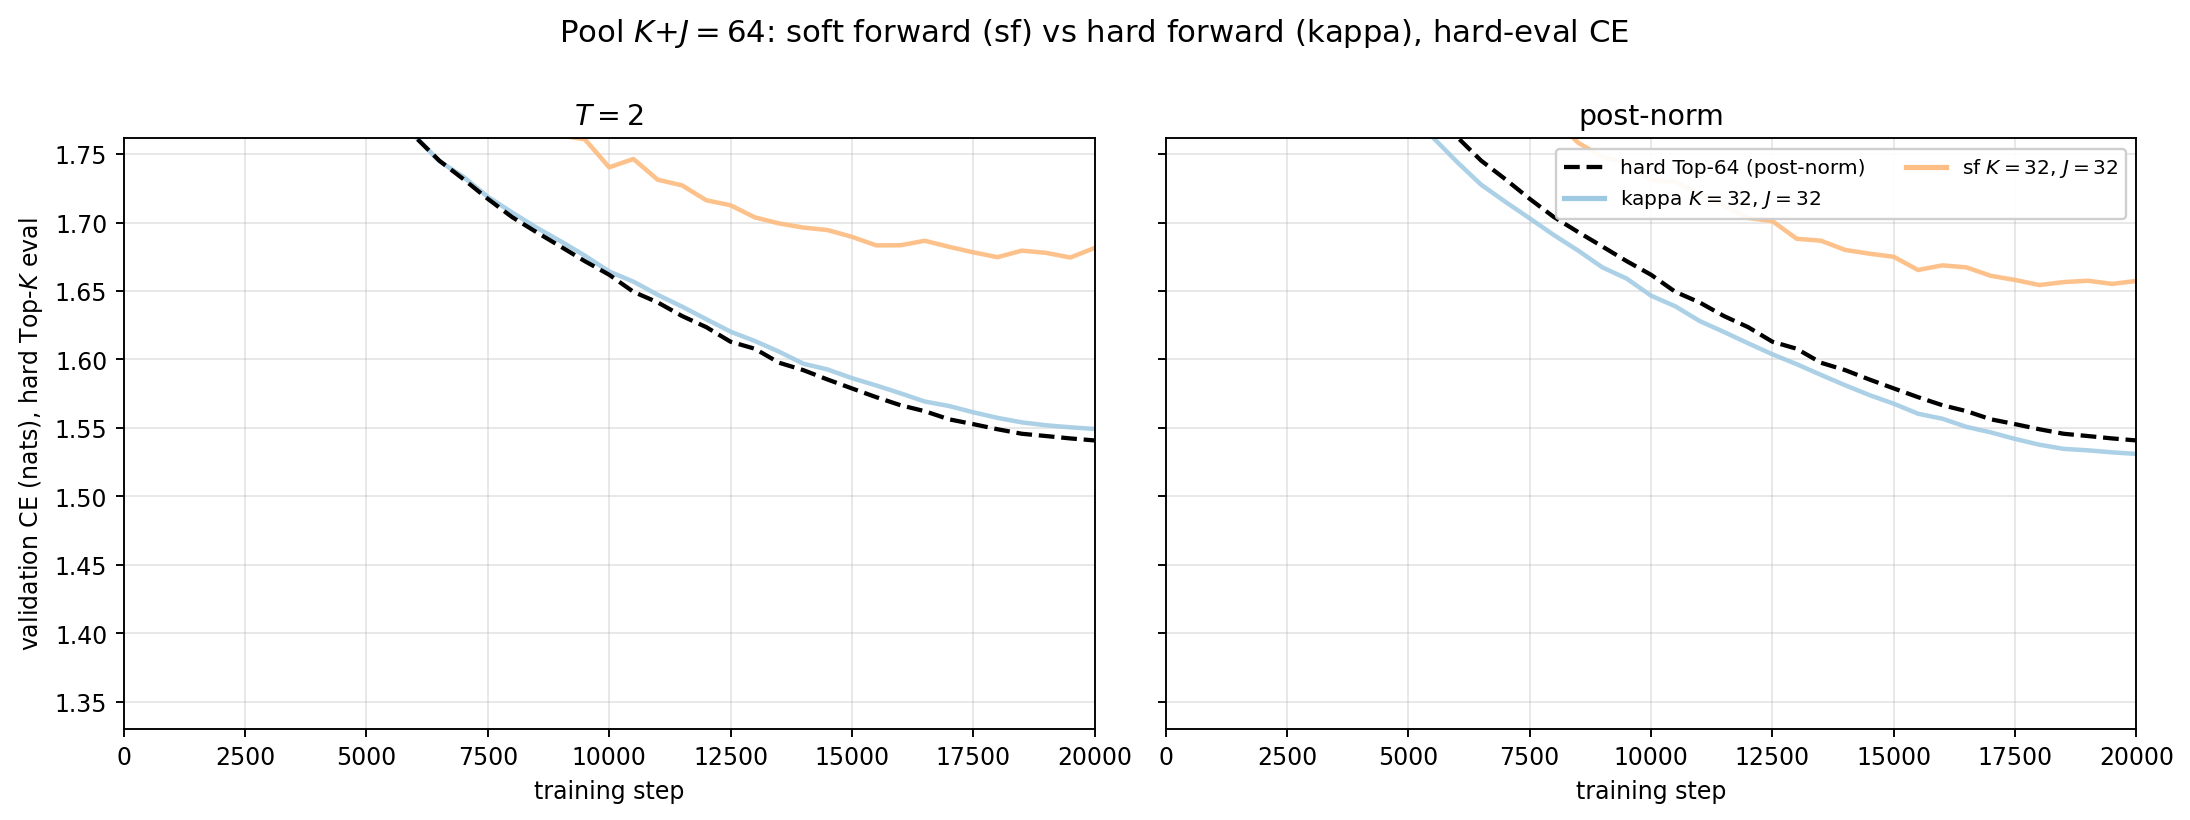
\includegraphics[width=\textwidth]{figures/sf/sf_pool_k64.png}
\caption{Pool $\Kp=64$. The single cell $(32,32)$: the soft model's hard-eval
curve runs $\sim0.13$ nats above its twin in both variants.}
\end{figure}

\begin{figure}[htb]\centering
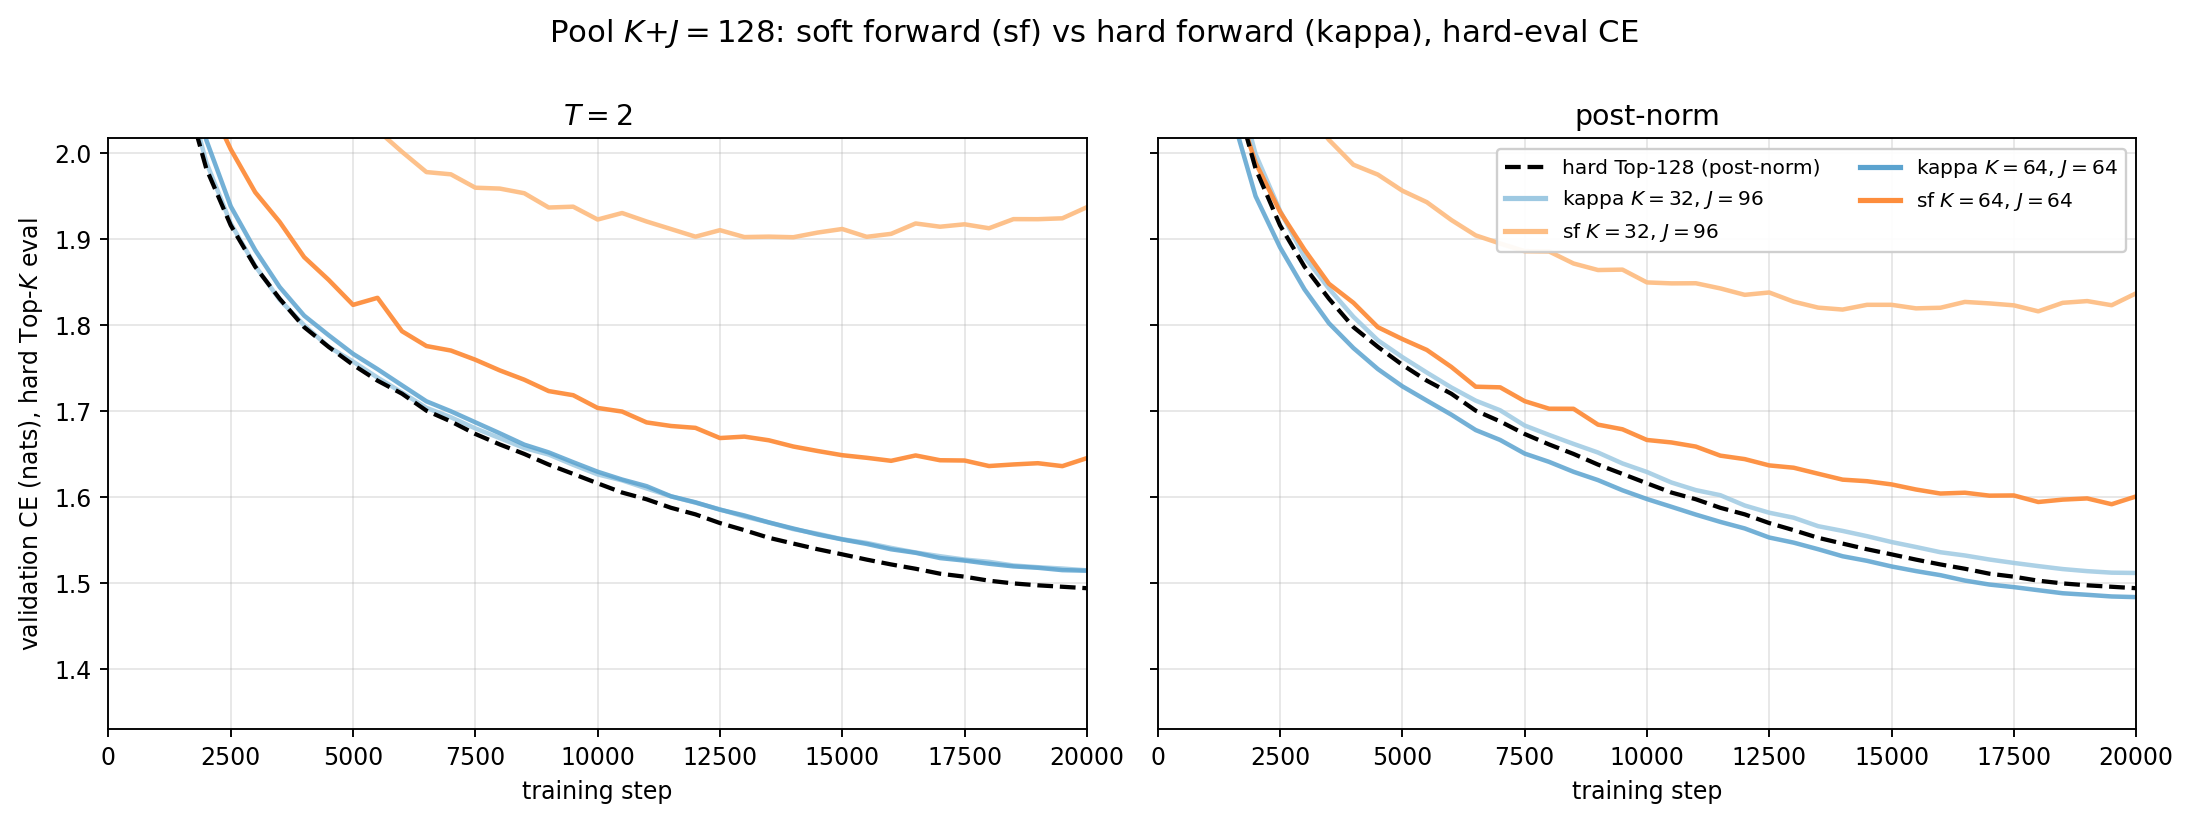
\includegraphics[width=\textwidth]{figures/sf/sf_pool_k128.png}
\caption{Pool $\Kp=128$. The $T=2$ soft cells drift \emph{upward} over the
second half of training as the tail mass grows; the post-norm holds flat but
offset. The kappa family and the hard baseline are unchanged from the earlier
note.}
\end{figure}

\begin{figure}[htb]\centering
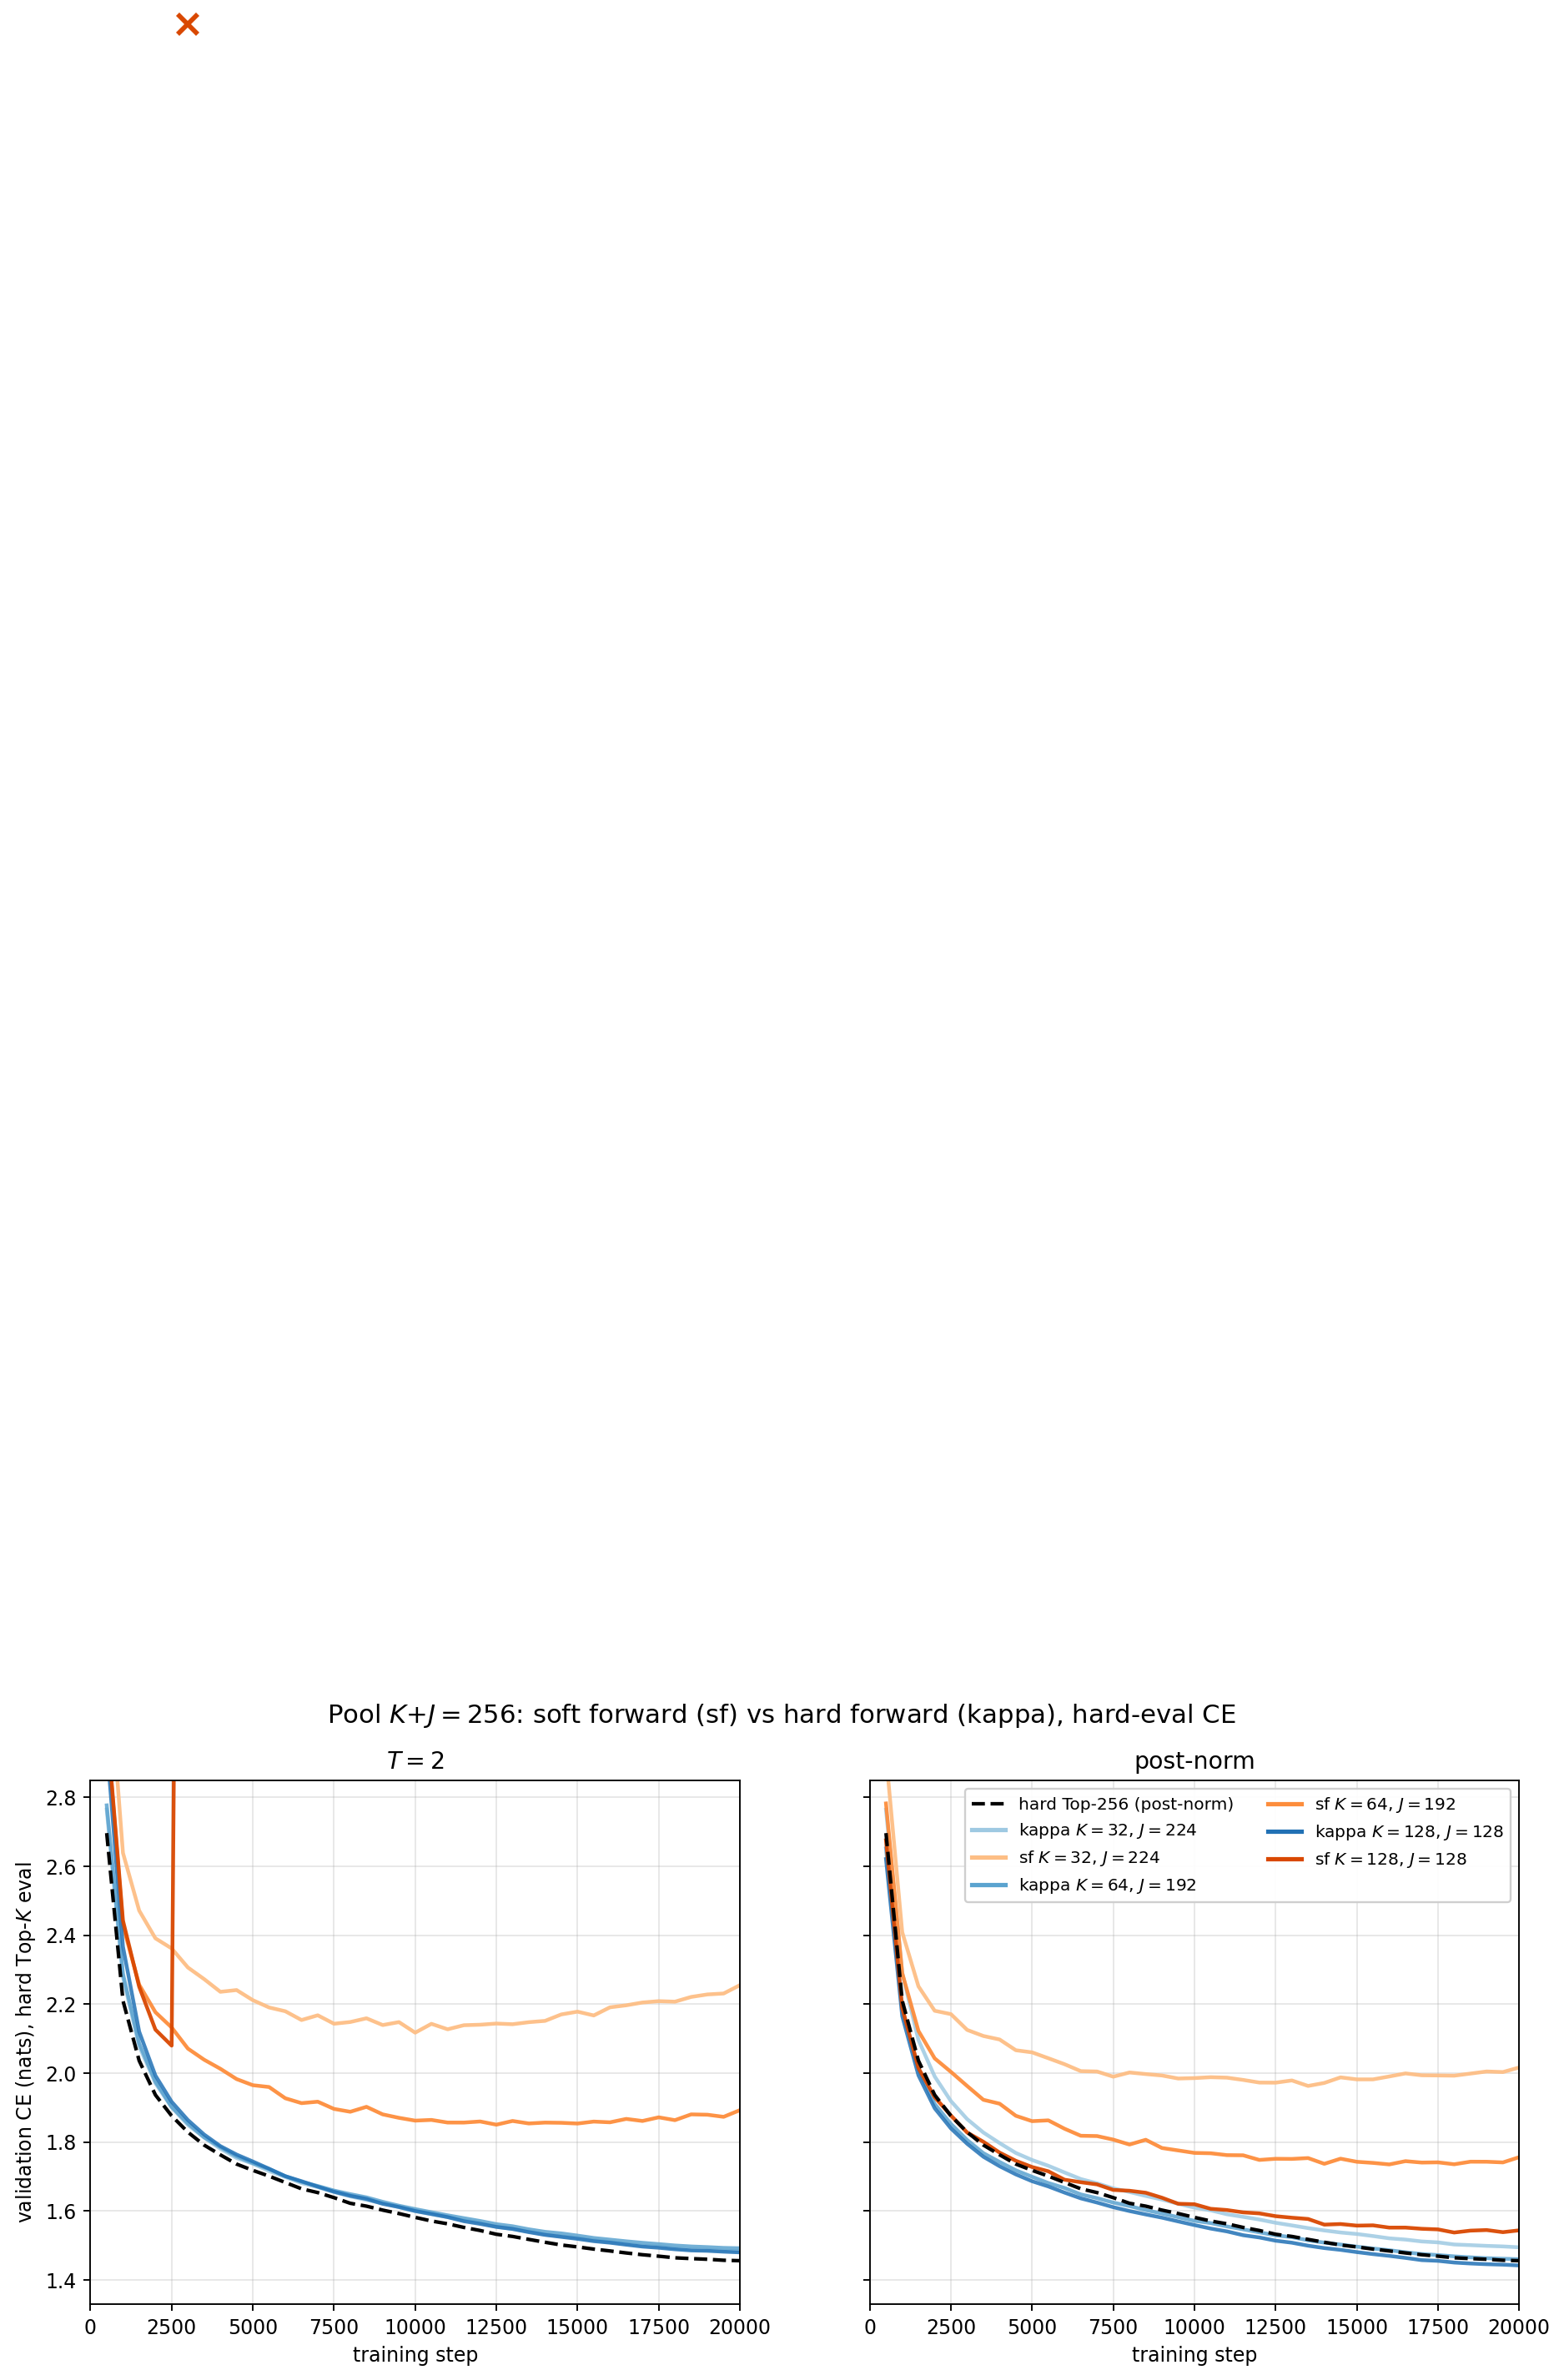
\includegraphics[width=\textwidth]{figures/sf/sf_pool_k256.png}
\caption{Pool $\Kp=256$. The soft $T=2$ cell at $(128,128)$ ends at its
guard stop (cross). Hard-eval damage orders inversely with $K$ in both
variants.}
\end{figure}

\begin{figure}[htb]\centering
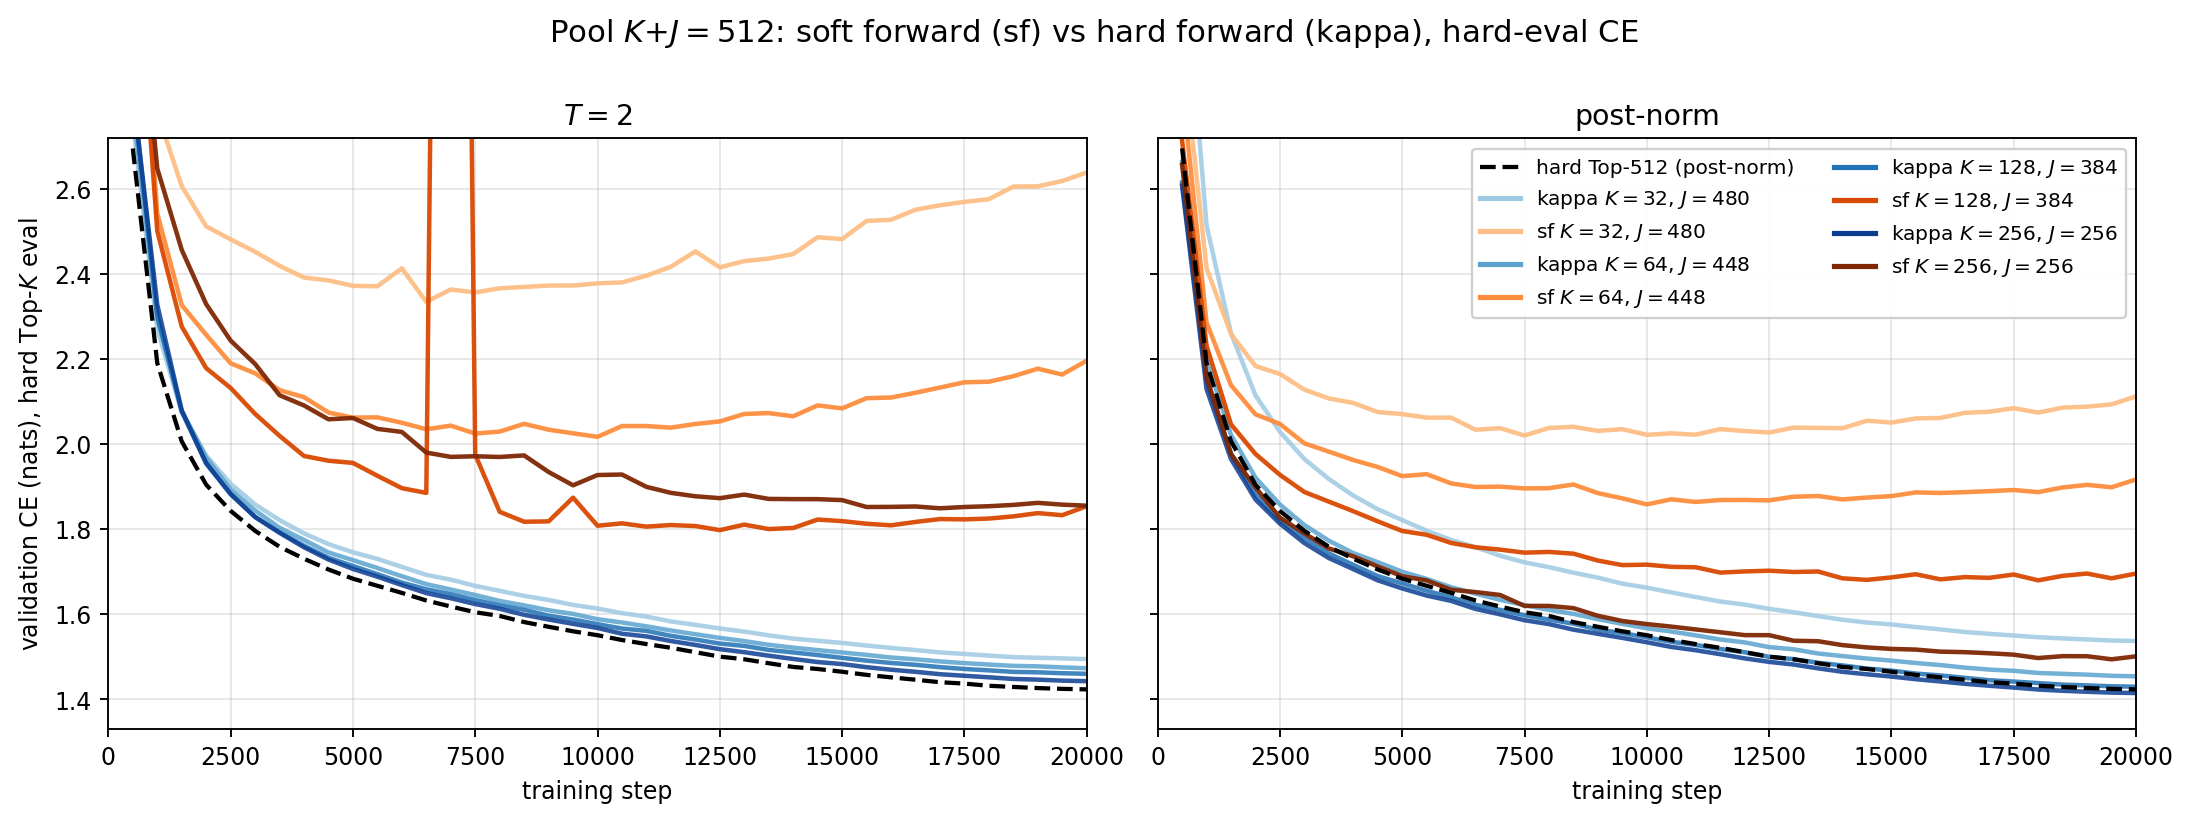
\includegraphics[width=\textwidth]{figures/sf/sf_pool_k512.png}
\caption{Pool $\Kp=512$. The widest windows: the soft family sits
$0.09$--$1.1$ nats above the blue twins under hard eval, with the $(128,384)$
$T=2$ excursion near step 7000 visible; the recovered curve returns to its
trend.}
\end{figure}

\begin{figure}[htb]\centering
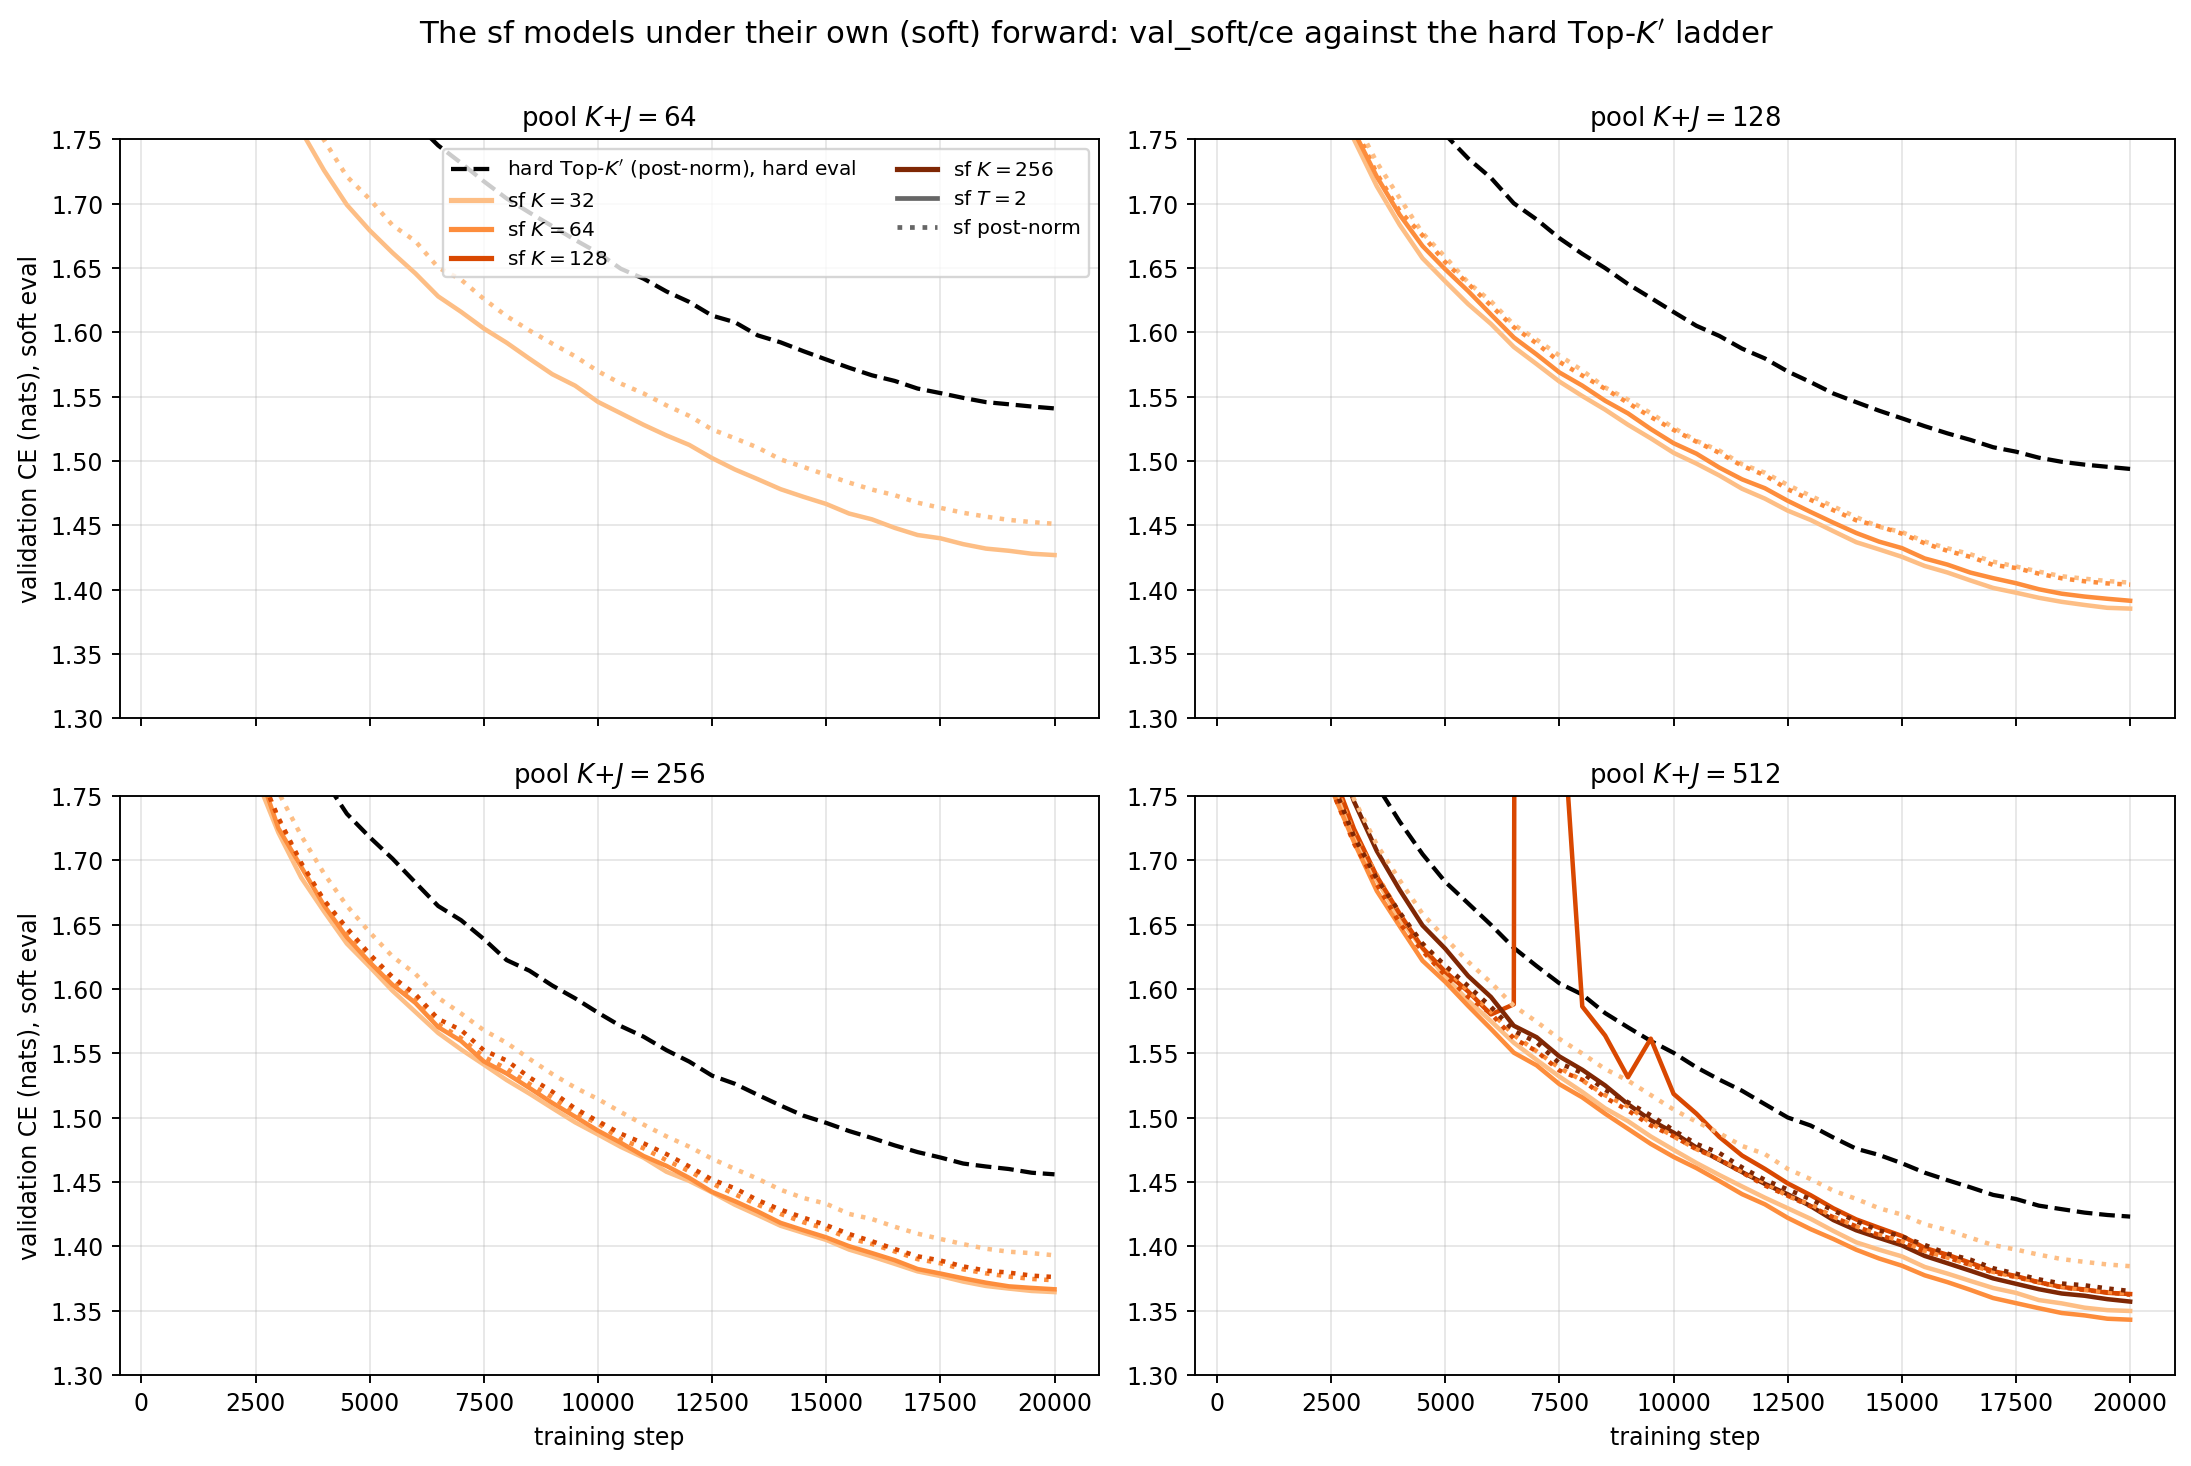
\includegraphics[width=\textwidth]{figures/sf/sf_soft_eval.png}
\caption{The soft family under its own forward (\code{val\_soft/ce}), one
panel per pool, against the pool-matched hard Top-$\Kp$ baseline (dashed).
Solid $T=2$, dotted post-norm. Every curve ends below the dashed reference;
within a panel the curves cluster tightly across $K$.}
\end{figure}

% ============================================================
\section{Interpretation}
% ============================================================

The two evaluations measure different models, and the tables say the trained
one is good and the hardened one is not. Training optimizes the weighted-pool
forward, and the optimizer uses the freedom this buys: it parks measurable
probability mass on the $J$ tail features ($3$--$93$ per-token units of
$\sum p$ beyond $K$), and the task loss of the trained function improves with
every widening of the pool -- past the point where the hard-forward family
reverses, and below every hard baseline with the same pool. Hard evaluation
then deletes exactly that mass, and the measured damage is proportional to it
within each $K$. Nothing here is surprising once stated this way; the
quantitative point is that the exchange rate is poor everywhere in the grid:
even the best cell pays $+0.086$ nats for hardening, which is more than the
entire margin the hard-forward surrogate holds over hard Top-$\Kp$.

The inverted orderings follow from the same picture. A wider kernel ($T=2$)
fattens $p$ in the tail, which is capacity under soft evaluation and liability
under hard; the post-norm, which controls the score scale rather than the
kernel, keeps the profile sharper -- better hardened, worse soft. At a fixed
pool the active count $K$ mostly relabels which features sit above the
boundary reference without changing the pool's capacity, so the soft loss
barely moves with $K$ while the hard loss moves strongly.

Read as a design, \code{rblapsum\_sf} at these settings is a LapSum-style
soft bottleneck with a rank-defined boundary and no barrier solve, trained
exactly as evaluated. On that reading it is the best model in the project at
every pool size, and the natural follow-ups are the ones that would close the
train/inference gap rather than compare it to hard models it does not
implement: annealing $T$ toward a hard forward over training, a hardening
fine-tune phase, or an explicit penalty on the tail mass
(\code{rb\_soft\_mass} is already the right observable, and its correlation
with the hard-eval gap suggests a target). None of these were run.

% ============================================================
\section{Scope}
% ============================================================

All cells are single runs at one seed, and the hard-forward references are
reused from the earlier campaigns rather than retrained -- identical configs
and seed, but a different machine (5090s against 4090s), so bit-level
reproduction is not implied. The soft-forward evaluation exists only for the
new family; the hard baselines have no soft variant to compare against. Only
one boundary mode (\code{through\_rank\_kappa}) and support scale ($1.0$) were
trained; the ablations the mode switches were built for -- \code{detach},
\code{through\_rank}, scaled boundary terms -- are untouched. The divergence
at $(128,128)$, $T=2$ is a single cell and earlier work found marginal-cell
divergence to be stochastic, so it should be read as a rate, not a verdict.
Finally, the soft model's inference-time cost differs from a hard Top-$K$
model's: its forward keeps $K{+}J$ weighted features, so comparisons at
matched $K$ favour it unfairly on quality and disfavour it on sparsity; the
pool-matched comparison in the second table is the fair one.

\end{document}
